% !TeX root = ../index.tex
\chapter{Project Management}

The project will be using Git for source code management and the web-based repository hosted on the GitHub service. GitHub also provides bug tracking and task management which will be used to track the progress of this coursework. The project can be found on GitHub at \url{https://github.com/wopian/hibari-api}

GitHub Projects will be used to track the development of the web service and the report as two separate projects. Each project is then broken down into "Epics" using the Milestones feature. Tasks to complete, or sprints, are tracked using the issues feature - which can be labelled to provide useful information (e.g a bug or feature) and assigned to a project and milestone. Issues can be further broken down into sub-tasks to ensure everything related to the issue has been completed.

The projects feature also allows assigning a status to each issue, where it can be changed between "To Do", "In Progress" and "Done". In the progress bars these are shown as grey, purple and green respectively.

\begin{figure}[H]
  \caption{GitHub Projects}
  \centering
  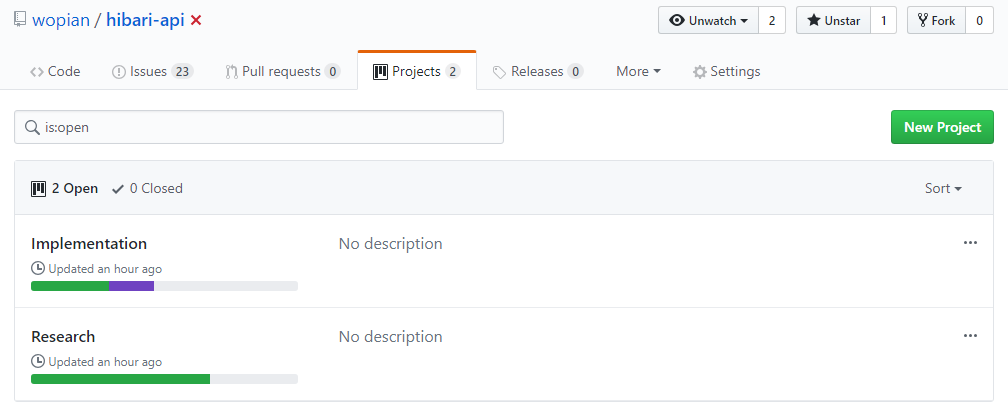
\includegraphics[width=\textwidth]{3-projects}
\end{figure}

\begin{figure}[H]
  \caption{GitHub Milestones}
  \centering
  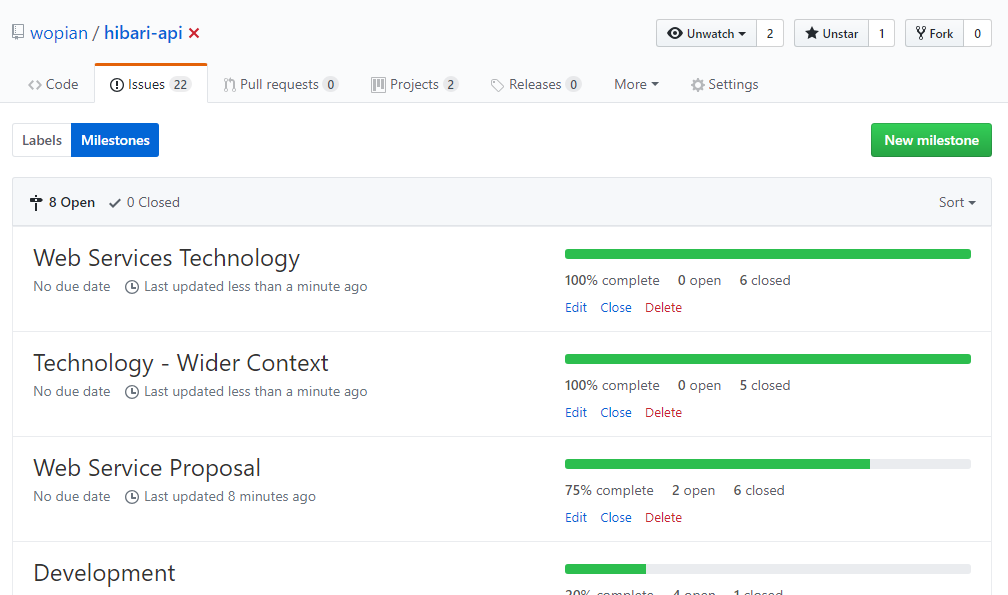
\includegraphics[width=\textwidth]{3-milestones}
\end{figure}

\begin{figure}[H]
  \caption{GitHub Issues}
  \centering
  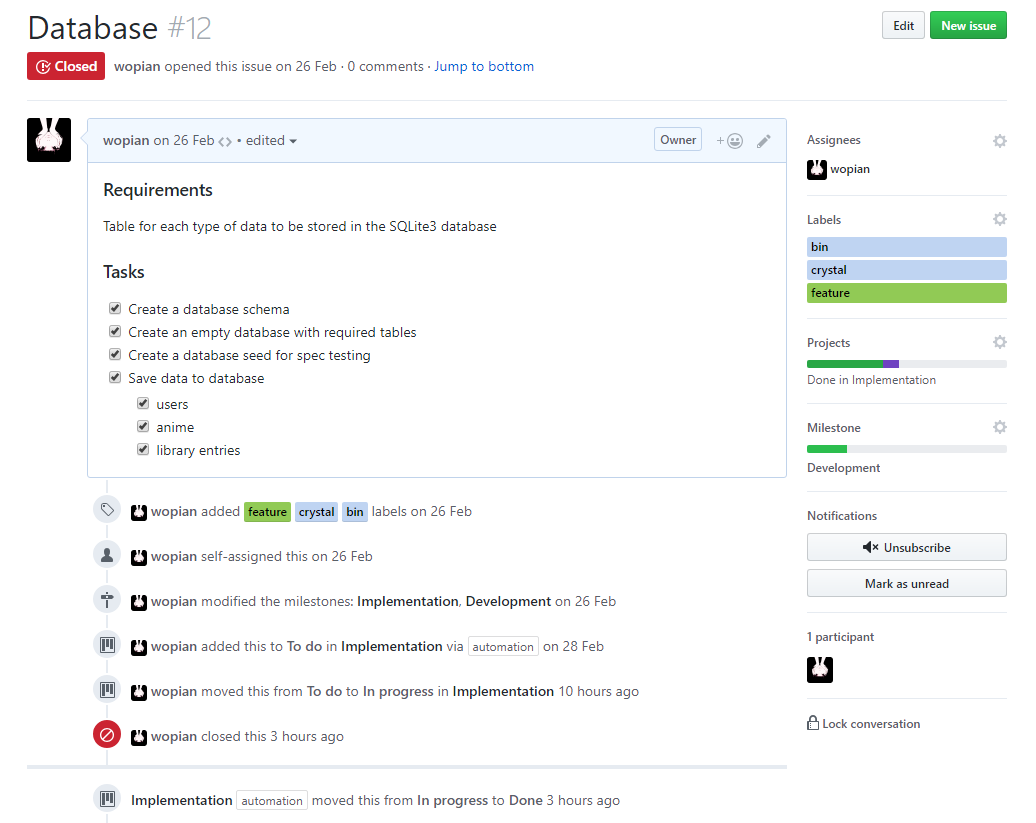
\includegraphics[width=\textwidth]{3-issues}
\end{figure}
